\documentclass{sig-alternate-05-2015}
\usepackage{amsmath}
\usepackage{amssymb}
\DeclareMathOperator*{\argmax}{argmax}
\DeclareMathOperator*{\argmin}{argmin}

\usepackage{mathrsfs}

\begin{document}

\setcopyright{acmcopyright}

\title{Improving Collaborative Filtering with\\
Long-Short Interest Model}

%\numberofauthors{1}
%\author{
%\alignauthor
%Chao Lv \quad
%Lili Yao \quad
%Yansong Feng \quad
%Dongyan Zhao\titlenote{Corresponding author.}\\
%\affaddr{Institute of Computer Science and Technology}\\
%\affaddr{Peking University, Beijing 100871, China}\\
%\email{\{lvchao, yaolili, fengyansong, zhaodongyan\}@pku.edu.cn}
%}

\maketitle

\begin{abstract}
Collaborative filtering (CF) has been widely employed within
recommender systems in many real-world situations.
The basic assumption of CF is that items liked by the same user would be similar and
users like same items would share similar interest.
But it is not always true since the user's interest changes over time.
It should be more reasonable to assume that
if these items are liked by the same user in the same time period,
there is a strong possibility that they are similar,
but the possibility will shrink if the user likes they in different time period.
In this paper, we propose a long-short interest model (LSIM) based on
the new assumption to improve collaborative filtering.
In special, we introduce a neural network based language model
to extract the sequential features on user's preference over time.
Then, we integrate the sequential features to solve the rating prediction task
in a feature based collaborative filtering framework.
Experimental results on three MovieLens datasets demonstrate that
our approach can achieve the state-of-the-art performance.
\end{abstract}

%\category{H.3.3}{Information Search and Retrieval}{Information Filtering}
%\category{H.2.8}{Database Management}{Data Mining}

\begin{CCSXML}
	<ccs2012>
	<concept>
	<concept_id>10010520.10010521.10010542.10010294</concept_id>
	<concept_desc>Computer systems organization~Neural networks</concept_desc>
	<concept_significance>500</concept_significance>
	</concept>
	<concept>
	<concept_id>10002951.10003317.10003347.10003350</concept_id>
	<concept_desc>Information systems~Recommender systems</concept_desc>
	<concept_significance>500</concept_significance>
	</concept>
	</ccs2012>
\end{CCSXML}

\ccsdesc[500]{Computer systems organization~Neural networks}
\ccsdesc[500]{Information systems~Recommender systems}

\printccsdesc

\keywords{Recommender System; Collaborative Filtering; Long-Short Interest Model;}

\section{Introduction}
In the modern era of information overload,
recommender system (RS) has become more and more popular in many real-world situations.
Recommender system aims to help users find the items,
they are more likely to be interested in,
from huge amounts of candidates.
Lots of websites (e.g. Amazon, Netflix, Alibaba and Hulu) use recommender system to
target customers and provide them with useful information.
An excellent recommendation system can effectively increase the amount of sales.
For instance, 80\% of movies watched on Netflix
come from their recommender system \cite{gomez2015netflix}.

A widely used setting of recommender system \cite{ricci2011introduction} is to
predict the rating a user will evaluate on a new item (such as a movie)
given the past rating history of the users.
Lots of classical recommendation methods have been proposed
during the last decade, and they can be categorized into two classes:
content based methods and collaborative filtering based methods.
Content based methods \cite{pazzani2007content} take advantage of
user profiles and item properties for recommendation.
While collaborative filtering based approaches \cite{su2009survey} utilize
the past interactions or preferences, such as users' ratings on items,
without using user or product content information for recommendation.
Collaborative filtering based approaches have attracted more attention
due to their impressive performance, and developed for many years and
keep to be a hot area in both academia and industry.

\begin{figure}[htbp]
    \centering
    \includegraphics[scale=0.7]{images/example.pdf}
    \caption{The preference records of user whose id is $5988$ in MovieLens-1M dataset,
    which are sorted by their rated time.}
    \label{fig:example}
\end{figure}

Collaborative filtering assumes that items liked by the same user would be similar and
users like same items would share similar interest.
However, it is not always true because the user's interest changes over time.
For example, given a user in MovieLens-1M dataset whose id is $5988$,
Figure \label{fig:example} shows the movies he watched sorted by the rating time.
We can find that this user liked watching comedy movies in April 2004 and
changed to love watching drama movies in June 2004.
These movies are going to be treated similar in conventional collaborative filtering,
but they are not in actual.
A more reasonable assumption, aka long-short interest assumption, should be that
items liked by the same user in the same time period have a higher possibility
to be similar than items liked by the same user in different time period.

\begin{figure*}[htbp]
    \centering
    \includegraphics[scale=0.38]{images/example2.pdf}
    \caption{Paragraph2vec learns vector representations of sentences and words
    based on the word order
    while LSIM extracts sequential features of users and items
    based on the rating order.
    }
    \label{fig:example2}
\end{figure*}

Inspired by paragraph2vec algorithm \cite{le2014distributed} for
learning vector representations of words which take advantage of
a word order observed in a sentence,
we introduce a long-short interest model (LSIM) to extract sequential features
of users and items based on the new assumption.
As illustrated in Figure \ref{fig:example2}, user is similar with the sentence,
both of them contains a sequence follow some order,
and items are similar with words because both of them follow the law
that the more close they are, the more similar they are.
To verify the effectiveness of the learned sequential features of users
and items, we integrate them as side information to solve the rating prediction task
in a feature based collaborative filtering framework.

The main contributions of this paper include:
(1) We introduce a long-short interest model (LSIM) to extract sequential features
of users and items based on the long-short interest assumption.
(2) We demonstrate the effectiveness of the sequential features
via integrating them as side information to solve the rating prediction task.
(3) Experiments on three public MovieLens shows LSIM can achieve the state-of-the-art performance.

The rest of the paper is organized as follows. Section 2 gives an overview of the related work.
Then, we describe our long-short interest model and the feature based collaborative filtering
framework in Section 3. The experimental results as well as the comparisons with
baseline system are shown in Section 4.
Finally, we conclude the paper and outline our future work in Section 5.

\section{Related Work}
Our work is closely related to collaborative filtering and
neural network language model.
We will discuss them in the following subsections.

\subsection{Collaborative Filtering}
Collaborative filtering based methods can mainly divided into three categories:
user-based collaborative filtering, item-based collaborative filtering and
model-based collaborative filtering.
User-based collaborative filtering \cite{resnick1994grouplens} recommends
items liked by users who are similar with you
while item-based collaborative filtering \cite{sarwar2001item} aims to
recommend items similar with ones you liked in the past.
Matrix factorization (MF) is the most popular model-based collaborative filtering methods,
their success at the Netflix competition \cite{koren2009matrix, bennett2007netflix}
have demonstrated their amazing strength,
and lots of variants of it have been proposed in the following works.

Basically, the given ratings matrix $\mathbf{R} \in \mathbb{R}^{N*M}$
consisting of the item preferences of the users can be decomposed as
a product of two low dimensional matrices $\mathbf{U} \in \mathbb{R}^{N*K}$
and $\mathbf{V} \in \mathbb{R}^{K*M}$.
$\mathbf{U}$ could be treated as a user-interest matrix while
$\mathbf{U}$ could be treated as a item-interest matrix.
$K$ is the amount of interest.
The decomposition can be carried out by a variety of methods
such as singular value decomposition (SVD) based approaches \cite{mazumder2010spectral},
non-negative matrix factorization approach \cite{lee2001algorithms}
and regularized alternative least square (ALS) algorithm \cite{zhou2008large}.
Meanwhile, non-linear algorithms are proposed to catch subtle factors,
such as Non Linear Probabilistic Matrix Factorization \cite{lawrence2009non},
Factorization Machines \cite{rendle2010factorization} and
Local Low Rank Matrix Approximation \cite{lee2013local}.
However, these methods group users and treat items they rated equally,
which will lose the sequential features to describe the long-short interest.

Matrix factorization methods suffer from the cold start problem,
i.e. what recommendations to make when a new user/item arrives in the system.
Another problem often presented in many real world applications is data sparsity.
Incorporating side information has shown promising performance
in collaborative filtering in such scenarios.
In recent years, deep learning \cite{hinton2006reducing, hinton2006fast}
has attracted a lot of attention due to its amazing performance
to learn representations on various tasks,
especially in computer vision and natural language processing.
Hence, some works make use of deep learning to learn effective
features from side information to improve the performance of recommender system,
such as \cite{salakhutdinov2007restricted, van2013deep, wang2015collaborative, li2015deep}.

Neural Networks have attracted little attention in the collaborative filtering community.
Salakhutdinov \textit{et al.} \cite{salakhutdinov2007restricted} were the first
work to tackle the Netflix challenge using Restricted Boltzmann Machines (RBM).
They modified the RBM as a two-layer undirected graphical model
consisting of binary hidden units and softmax visible units,
and tested their model on the Netflix dataset and
showed a comparable result with the start-of-the-art.
On music recommendation, Van \textit{et al.} \cite{van2013deep}
directly use Convolutional Neural Network (CNN) to learn effective representations
of songs and use them in content-based collaborative filtering framework.
Wang \textit{et al.} \cite{wang2015collaborative} 
directly coupled matrix factorization with deep learning models,
and proposed a hierarchical Bayesian model called Collaborative Deep Learning (CDL)
which tightly couples Stacked Denoising AutoEncoders (SDA) \cite{vincent2008extracting} and
Collaborative Topic Regression (CTR) \cite{wang2011collaborative} to solve the cold start problem.
Li \textit{et al.} \cite{li2015deep} proposed a generate learning framework
to combine rating matrix and side information, they used 
Probabilistic matrix factorization (PMF) \cite{salakhutdinov2011probabilistic} and
marginalized Stacked Denoising AutoEncoders (mSDA) \cite{chen2012marginalized}
in their approach, which is close to CDL but more efficient and scalable.
Meanwhile, their model can learn deep features for both items and users
while CDL only extracts deep features for items.
In our work, although sequential features learned by LSIM are used as side information
in the feature based collaborative framework, but actually they aims to describe
the long-short interest, and can't be utilized to solve the cold start problem.

\subsection{Neural Network Language Model}
Traditional language model uses a one-hot representation to represent each word
as a feature vector, where these feature vectors have the same length as the size
of vocabulary, and the position that corresponds to the observed word is equal to 1,
and 0 otherwise. However, this approach often exhibits significant limitations
in practical tasks, suffering from high dimensionality and severe data sparsity.

Mikolov \textit{et al.} \cite{mikolov2013efficient, mikolov2013distributed} proposed
the word2vec algorithm to address these issues. They take advantage of the word order
in text documents, explicitly modeling the assumption that closer words in the word
sequence are statistically more dependent, and have generalized the classic n-gram
language models by using continuous variables to represent words in a vector space.
The continuous bag-of-words (CBOW) and skip-gram (SG) language models are highly
scalable for learning word representations from large-scale corpora.
The word2vec algorithm breaks the semantic gap between words.
For example, ``trade'' and ``deal'' are totally different words in the one-hot representation,
but they are similar in word2vec distribution representation.
Le \textit{et al.} \cite{le2014distributed} followed the above work and proposed
the paragraph2vec algorithm to simultaneously learn vector representations of sentence
and words by considering the sentence as a ``global context".
Our long-short interest model shares similar idea with paragraph2vec algorithm,
but we aim to simultaneously learn vector representations of user and items
correspondingly by considering the user as a ``global context".

\section{Our Approach}
In this section,
we first describe the definition of the rating prediction task and
the notation we are going to use in this paper.
Then we introduce our long-short interest model to extract the sequential features
of users and items based on the long-short interest assumption.
In the last, we utilize the sequential features as side information
in the feature based collaborative filtering framework to make the final prediction.

\subsection{Problem Definition}
Given $N$ users and $M$ items, the rating $r_{ij}$ is the rating given by
the $i^{th}$ user for the $j^{th}$ item.
In the common real-world situations,
users usually rate on a fraction of items, not on the whole items.
Therefore,
those ratings entail a big and sparse matrix $\mathbf{R} \in \mathbb{R}^{N \times M}$.
The goal of recommender system is to make a prediction on the missing ratings.
Based on that, we will know the preference of a user on the items he never rates,
and recommend high score items to him.

Matrix Factorization is a classic method to solve this problem.
It aims to find a $K$ dimensional low rank matrix $\mathbf{\hat{R}} \in \mathbb{R}^{N \times M}$
where $\mathbf{\hat{R}} = \mathbf{U} \mathbf{V}^\mathrm{T}$ with
$\mathbf{U} \in \mathbb{R}^{N \times K}$ and $\mathbf{V} \in \mathbb{R}^{M \times K}$
are two matrices of rank $K$ encoding a dense representation of the users and items with

\begin{equation}
\begin{aligned}
	\argmin_{\mathbf{U},\mathbf{V}}
	\sum_{(i,j) \in \mathcal{K}(\mathbf{R})}
	&( r_{ij} - \vec{\mathbf{u}}_i^{\mathrm{T}} \vec{\mathbf{v}}_j ) ^ 2 + \\
	&\lambda ( \left\| \vec{\mathbf{u}}_i \right\|_{Fro}^2 +
	\left\| \vec{\mathbf{v}}_j \right\|_{Fro}^2 )
\end{aligned}
\end{equation}

where $\mathcal{K}(\mathbf{R})$ is the set of indices of known ratings,
$\vec{\mathbf{u}}_i$ and $\vec{\mathbf{v}}_j$
are the corresponding line vectors of $\mathbf{U}$ and $\mathbf{V}$,
$\lambda$ is the coefficient that controls the influence of L2 regularization,
and $\left\| \cdot \right\|_{Fro}$ is the Frobenius norm.

Table \ref{tab:notations} summarizes the symbols used in our approach.
In the next section, we will propose a long-short interest model
to extract sequential features of users and items based on the long-short interest assumption.

\begin{table}[htbp]
    \centering
    \caption{Summary of notations.}
    \label{tab:notations}
    \begin{tabular}{|c|l|}
        \hline
        \textbf{Notation} & \textbf{Description} \\
        \hline
        $N$ & Number of users \\
        $M$ & Number of items \\
        $K$ & Dimension of latent factors \\
        $D$ & Dimension of sequential features \\
        $\mathbf{R} \in \mathbb{R}^{N \times M}$ & Rating matrix \\
        $\mathbf{U} \in \mathbb{R}^{N \times K}$ & Latent factors of users \\
        $\mathbf{V} \in \mathbb{R}^{M \times K}$ & Latent factors of items \\
        $\mathbf{X} \in \mathbb{R}^{N \times D}$ & sequential features of users \\
        $\mathbf{Y} \in \mathbb{R}^{M \times D}$ & sequential features of items \\
        \hline
    \end{tabular}
\end{table}

\subsection{Long-short Interest Model}
Collaborative filtering aims at estimating the ratings a user is going to give to
all other items he never interact with by using the ratings of all the other users.
The basic assumption of collaborative filtering is that items liked by the same user
would be similar or users like same items would share similar interest.
However, in real-world situations, it is not always true because users' interest
may change over a long time period.
Meanwhile, the interest distribution of a user in a fixed time period
are stable and don't change too much.

To describe this phenomenon that interest changes over a long time period but
keep stable in a short time period,
we propose the definition of \textbf{long interest} and \textbf{short interest}.

\begin{itemize}
\item \textbf{long interest} reflects the interest distribution of a user
in a long time period, and it is reflected in the whole items list of the user's preference.
\item \textbf{short interest} reflects the interest distribution of a user
in a short time period, and it is reflected in a fraction of the whole items list of
the user's preference in a fixed length sliding window.
\end{itemize}

Under this definition, each user will have a long interest, and each long interest will
correspond several short interest. At the same time,
we propose two assumption based on long interest and short interest.

\begin{enumerate}
\item items liked in the same short interest of the same long interest have a higher
possibility to be similar than ones liked in different short interest of the same long interest.
\item the more times items show in the same short interest of different long interest,
the higher possibility they are similar.
\end{enumerate}

\begin{figure}[htbp]
	\centering
	\includegraphics[scale=0.5]{images/embedding.pdf}
	\caption{A Example for Short Interest and Long Interest}
	\label{fig:embedding}
\end{figure}

For example, as illustrated in the top of Figure \ref{fig:embedding},
given a certain $\mathbf{user}$, we can see five items
$\mathbf{item1}$, $\mathbf{item2}$, ..., $\mathbf{item5}$, he liked in the last,
are list on the timeline according to the liked time order.
Those items compose the long interest of this $\mathbf{user}$.
Let's assume that the time window size of short interest is set to $2$,
That means $\mathbf{item1}$ and $\mathbf{item2}$ are in the same short interest,
$\mathbf{item2}$ and $\mathbf{item3}$ are in the same short interest, and so on.
Meanwhile $\mathbf{item2}$ and $\mathbf{item5}$ are in different short interest.
Therefore $\mathbf{item2}$ has a higher possibility to be similar with $\mathbf{item1}$
than $\mathbf{item5}$ based on our long-short interest assumption.

In special, we embed users and items into a low dimensional space
to characterize these similarity in mathematical sense.
We use European space distance between items in this low dimensional space
to represent the similarity between them.
Hence, $\mathbf{item2}$ has a higher possibility to be similar with $\mathbf{item1}$
than $\mathbf{item5}$ means $\mathbf{item2}$ is close to $\mathbf{item1}$ and far away from $\mathbf{item5}$
in this low dimensional space, as shown in the bottom of Figure \ref{fig:embedding}.

\begin{figure}[htbp]
	\centering
	\includegraphics[scale=0.55]{images/doc2vec.pdf}
	\caption{Embedding Model for Extracting Interest Similarity from Users and Items}
	\label{fig:doc2vec}
\end{figure}

Inspired by paragraph2vec algorithm \cite{le2014distributed} for learning
vector representations of words which take advantage of a word order observed in a sentence,
we introduce a neural network based language model to carry out the embedding of sequential features.
The embedding model simultaneously learns vector representations of users and items
by considering the user as a global context,
and the architecture of the embedding model is illustrated in Figure \ref{fig:doc2vec}.

The training data set was derived from users interaction timeline $T$,
which comprises users $x_i (i=1,2,...,N)$ and their interacted items ordered by the interacted time,
$y_{i_1}$, $y_{i_2}$, ..., $y_{i_{L_i}}$
\footnote{we use symbol $x$ and $y$ instead of classic $u$ and $v$ to avoid confusion between $v$
and vector symbol $\mathbf{v}$ in neural network language model.},
where $L_i$ denotes number of items interacted by user $x_i$,
which is much less than the amount of items $M$.
To characterize the \emph{long interest}, we consider the whole items list as the context and generate
the long interest of the current user.
To characterize the \emph{short interest}, we consider items in the same local interest as the context
and generate items in it one by one with the help of long interest.
More formally, objective of the embedding model is to
maximize the log-likelihood over the set of $T$ of all the interaction timeline,

\begin{equation}
\begin{aligned}
	\sum_{i=1}^{N} \bigg( &p(x_i | y_{i_1}, y_{i_2}, ..., y_{i_{L_i}}) + \\
	                      &\sum_{j=1}^{L_i} p(y_{i_j} | y_{i_{j-c}} : y_{i_{j+c}}, x_i) \bigg)
\end{aligned}
\end{equation}

where $c$ is the time window size, $y_{i_{j-c}} : y_{i_{j+c}}$ denotes the sequence
$y_{i_{j-c}}, y_{i_{j-c+1}}, ..., y_{i_{j+c}}$ excluding $y_{i_j}$.

$p(x_i | y_{i_1}, y_{i_2}, ..., y_{i_{L_i}})$ is the probability to generate
the long interest of $u_i$ based on all items he interacted.
The prediction task is typically done via a multiclass classifier,
such as softmax. There, we have

\begin{equation}
	p(x_i | y_{i_1}, y_{i_2}, ..., y_{i_{L_i}}) =
	\frac
	{
		exp ( \overline{\mathbf{v}}_{1}^{\mathrm{T}} \mathbf{v}_{x_i}^{'} )
	}
	{
		\sum_{x^{'}} exp ( \overline{\mathbf{v}}_{1}^{\mathrm{T}} \mathbf{v}_{x^{'}}^{'} )
	}
\end{equation}

where $\mathbf{v}_{x_i}^{'}$ is the output vector representation of $x_i$,
and $\overline{\mathbf{v}}_{1}$ is averaged input vector representation of all the items
interacted by user $x_i$, i.e.

\begin{equation}
	\overline{\mathbf{v}}_{1} = \frac{\sum_{j=1}^{T_i} \mathbf{v}_{y_{i_j}}}{T_i}
\end{equation}

$p(y_{i_j} | y_{i_{j-c}} : y_{i_{j+c}}, x_i)$
is the probability to generate $y_{i_j}$ based on items in the same short interest
and the user's long interest. Similarly, using softmax multiclass classifier we have

\begin{equation}
	p(y_{i_j} | y_{i_{j-c}} : y_{i_{j+c}}, x_i) =
	\frac
	{
		exp( \overline{\mathbf{v}}_{2}^{\mathrm{T}} \mathbf{v}_{y_{i_j}}^{'} )
	}
	{
		\sum_{y^{'}} exp( \overline{\mathbf{v}}_{2}^{\mathrm{T}} \mathbf{v}_{y^{'}}^{'} )
	}
\end{equation}

where $\mathbf{v}_{y_{i_j}}^{'}$ is the output vector representation of $y_{i_j}$,
and $\overline{\mathbf{v}}_{2}$ is averaged input vector representation of items
int the same short interest and corresponding long interest $x_i$.

\begin{equation}
	\overline{\mathbf{v}}_{2} = \frac{
    \mathbf{v}_{x_i} + 
    \sum_{-c \leq k \leq c, k \not= 0}{\mathbf{v}_{y_{i_{j+k}}}}
    }{2c+1}
\end{equation}

Stochastic Gradient Descent (SGD) are used as the training method,
hierarchical softmax and negative sampling are two main approaches to accelerate
the computation, and we use negative sampling approach in this paper.

\subsection{Feature based Collaborative Filtering}
Feature based collaborative filtering \cite{chen2011feature, chen2012svdfeature} is a variety of
collaborative filtering, it allows us to build factorization models incorporating
side information such as temporal dynamics, neighborhood relationship,
and hierarchical information compare to conventional collaborative filtering,
it can also be capable of both rate prediction and collaborative ranking.

There are two kinds of side information in collaborative filtering:
user side information and item side information.
User side information could be the profiles of users, such as
gender, age and occupation.
Item side information is usually the properties of items,
it mainly depends on the recommendation sceneries.
In movie recommendation, item side information could be actor, director and genre
of the movie. In product recommendation, item side information could be the price
and category of the product.
Feature based collaborative filtering summarizes the two factors as feature vectors
(denoted by $\mathbf{u}_i \in \mathbb{R}^{n}$ and $\mathbf{v}_j \in \mathbb{R}^{m}$) and predicts
the preference score $\hat{r}$ as

\begin{equation}
\begin{aligned}
\hat{r}_{ij} = \sum_{k=1}^{n} \alpha_k \mathbf{u}_{ik} + &\sum_{k=1}^{m} \beta_k \mathbf{v}_{jk} + \\
&\left( \sum_{k=1}^{n} \mathbf{u}_{ik} \mathbf{p}_k \right) ^ \mathrm{T}
\left( \sum_{k=1}^{m} \mathbf{v}_{jk} \mathbf{q}_k \right)
\end{aligned}
\end{equation}

where $\alpha$ and $\beta$ controls the influence of each feature,
$\mathbf{p}_{k} \in \mathbb{R}^K$ and $\mathbf{q}_{k} \in \mathbb{R}^K$
are $K$ dimensional latent factors associated with each feature.
If we represent one-hot representation of users and items like

\begin{equation}
    \mathbf{u}_{ik} =
    \left\{
        \begin{aligned}
            1, &k = i \\
            0, &k \not= i
        \end{aligned}
    \right. \\
\end{equation}

\begin{equation}
    \mathbf{v}_{jk} =
    \left\{
        \begin{aligned}
            1, &k = j \\
            0, &k \not= j
        \end{aligned}
    \right. \\
\end{equation}

the equation for rating prediction will reduce to the basic matrix factorization

\begin{equation}
\hat{r}_{ij} = \alpha_i + \beta_j + \mathbf{p}_i ^ \mathrm{T} \mathbf{q}_j
\end{equation}

where $\alpha$, $\beta$ are the biases and $\mathbf{p}_i$, $\mathbf{q}_j$
are the latent factors for user $\mathbf{u}_i$ and item $\mathbf{v}_j$.

Various kinds of side information can be utilized to enhance these factors.
In some sense, the representation of users and items
learned from long-short interest model can be treated as a kind of side information,
because it distinguish the similarity and difference between users and items.

First, we define $\tilde{\mathbf{u}}_i$ as
the learned vector representation of users and $\tilde{\mathbf{v}}_j$ as
the learned vector representation of items.
Then, we get new features of users and items by add the learned vector representation
to origin one-hot representation.

\begin{equation}
    \mathbf{u}_{i} = \{ \mathbf{u}_{i} , \tilde{\mathbf{u}}_i \}
\end{equation}

\begin{equation}
    \mathbf{v}_{j} = \{ \mathbf{v}_{j} , \tilde{\mathbf{v}}_j \}
\end{equation}

There, the equation for rating prediction will change to

\begin{equation}
\begin{aligned}
\hat{r}_{ij} =
&\sum_{k=1}^{N+D} \alpha_k \{ \mathbf{u}_i , \tilde{\mathbf{u}}_i \}_k +
 \sum_{k=1}^{M+D} \beta_k  \{ \mathbf{v}_j , \tilde{\mathbf{v}}_j \}_k + \\
&\left( \sum_{k=1}^{N+D} \{ \mathbf{u}_i , \tilde{\mathbf{u}}_i \}_k \mathbf{p}_k \right) ^ \mathrm{T}
 \left( \sum_{k=1}^{M+D} \{ \mathbf{v}_j , \tilde{\mathbf{v}}_j \}_k \mathbf{q}_k \right) \\
= &\sum_{k=N+1}^{N+D} \alpha_k \tilde{\mathbf{u}}_{ik} +
 \sum_{k=M+1}^{M+D} \beta_k  \tilde{\mathbf{v}}_{jk} + \\
&\left( \sum_{k=N+1}^{N+D} \tilde{\mathbf{u}}_{ik} \mathbf{p}_k \right) ^ \mathrm{T}
 \left( \sum_{k=M+1}^{M+D} \tilde{\mathbf{v}}_{jk} \mathbf{q}_k \right) + \\
&\alpha_i + \beta_j + \mathbf{p}_i ^ \mathrm{T} \mathbf{q}_j
\end{aligned}
\end{equation}

where $N$ is the number of users, $M$ is the number of items,
$D$ is the dimension of sequential features of users and items learned from
our long-short interest model,
$\mathbf{p}_{k} \in \mathbb{R}^K$ and $\mathbf{q}_{k} \in \mathbb{R}^K$
are $K$ dimensional latent factors associated with each feature.

\section{Experiment}
In this section, we conduct several experiments to evaluate the effectiveness
of our proposed long-short interest model on three public
MovieLens \footnote{http://grouplens.org/datasets/movielens/} datasets.
In these experiments, we also conduct corresponding analysis to investigate:
(1) the rating prediction performance of our long-short interest model
compare to other benchmark models;
(2) the effect of our long-short interest model on users own different interaction number.

\subsection{Experimental Setup}
\subsubsection{Dataset}
We conduct experiments on three MovieLens datasets, i.e. MovieLens-1M,
MovieLens-10M and MovieLens-20M, which are commonly used for evaluating
collaborative filtering algorithms.

The MovieLens-1M dataset consists of about 1 million anonymous ratings of 3706 movies
made by 6040 MovieLens users who joined MovieLens in 2000,
and each rating is an integer between 1 (worst) and 5 (best).
Timestamp is represented in seconds and each user has at least 20 ratings.

The MovieLens-10M dataset contains about 10 million ratings and 95580 tags
applied to 10677 movies by 69878 users of the online movie recommender service MovieLens.
Users were selected at random for inclusion. All users selected had rated
at least 20 movies. Unlike previous MovieLens data sets, no demographic information is included.
Ratings are made on a 5-star scale, with half-star increments, i.e., 0.5 is the worst score
and 5.0 is the best score.

the MovieLens-20M dataset describes 5-star rating and free-text tagging activity.
It contains about 20 million ratings and 465564 tag applications across 26744 movies.
These data were created by 138493 users between January 09, 1995 and March 31, 2015.
This dataset was generated on March 31, 2015.
Users were selected at random for inclusion. All selected users had rated
at least 20 movies. No demographic information is included.
Each user is represented by an id, and no other information is provided.

These datasets also provide some side information about users and items,
such as gender, age and occupation of users and movies' genres,
but we don't use the side information in all our experiments.
Table \ref{tab:statistics} summarizes the statistics of three datasets.

\begin{table}[htbp]
    \centering
    \caption{Statistics of three MovieLens datasets and Netflix dataset.}
    \label{tab:statistics}
    \begin{tabular}{|l|c|c|c|c|}
        \hline
        \textbf{Dataset} & \textbf{\#Users} & \textbf{\#Items} & \textbf{\#Ratings} & \textbf{Sparsity} \\
        \hline
        ML-1M  & 6,040    & 3,706  & 1,000,209   & 95.53\% \\
        ML-10M & 69,878   & 10,677 & 10,000,054  & 98.66\% \\
        ML-20M & 138,493  & 26,744 & 20,000,263  & 99.46\% \\
        \hline
    \end{tabular}
\end{table}

\subsubsection{Metrics}
We employ two metrics, the Root Mean Square Error (RMSE) and the Mean Absolute Error (MAE),
to measure the rating prediction quality of our proposed approach in comparison with other
collaborative filtering based recommendation methods.
The metrics RMSE is defined as:

\begin{equation}
    RSME = \sqrt{ \frac{1}{N} \sum_{i,j} I_{ij} (R_{ij} - \hat{R}_{ij})^2 }
\end{equation}

where $R_{ij}$ denotes the ground-truth rating the user $i$ gives to the item $j$,
$\hat{R}_{ij}$ denotes the corresponding predicted rating the user $i$ gives to
the item $j$ by a method, $I_{ij}$ is a binary matrix that indicates the ratings
in the test set, and $N$ is the total number of ratings in the test set.
The metrics MAE is defined as:

\begin{equation}
    MAE = \frac{1}{N} \sum_{i,j} I_{ij} |R_{ij} - \hat{R}_{ij}|
\end{equation}

\subsection{Benchmark Models}
To demonstrate the superiority of our long-short interest model for rating prediction task,
we compare our model with several benchmark models.
In special, we use two popular toolkits, LibMF and LibFM, that are
widely used in both academia and industry as our benchmark models.

LibMF is an open source tool for approximating an incomplete matrix
using the product of two matrices in a latent space.
It provides solvers for real-valued matrix factorization,
binary matrix factorization, and one-class matrix factorization, and 
also supports parallel computation in a multi-core machine using CPU
instructions (e.g., SSE) to accelerate vector operations.
Its paper \cite{chin2015fast} won the best paper award in RecSys 2013.

Factorization machines (FM) are a generic approach that
allows to mimic most factorization models by feature engineering.
This way, factorization machines combine the generality of
feature engineering with the superiority of factorization models
in estimating interactions between categorical variables of large domain.
LibFM \cite{rendle2012factorization} is a software implementation
for factorization machines that features
Stochastic Gradient Descent (SGD) and
Alternating Least Squares (ALS) optimization as well as
Bayesian inference using Markov Chain Monte Carlo (MCMC).

\subsection{Overall Results}
In this section, we report the experimental results to demonstrate
the effectiveness of our long-short interest model.

The model proposed in LibMF toolkit is denoted as \textbf{LibFM},
the dimension of latent factors is set to $100$ and the number of
iterations is set to $1000$.

For the model proposed in LibFM, we denote the LibFM model optimized by
SGD as \textbf{LibFM-SGD}, the learn rate is set to $0.01$, the regular
parameter is set to $(0,0,0.01)$ and the stdev for initialization of 2-way
factors is set to $0.1$. Then we denote the LibFM model optimized by ALS
as \textbf{LibFM-ALS}, the regular parameter is set to $(0,0,10)$ and the
stdev for initialization of 2-way factors is set to $0.1$. Lastly, the
LibFM model optimized by MCMC is denoted as \textbf{LibFM-MCMC}, the stdev
for initialization of 2-way factors is set to $0.1$.

Meanwhile, we denote our long-short interest model as \textbf{LSIM},
the slide window size is set to $10$, the dimension of latent factors is
set to $256$ and the dimension of sequential features is set to $100$.
For feature based collaborative filtering framework, the learn rate is set
to $0.005$ and the regular parameter is set to $0.024$ for both users and items.

We split the rating data in each dataset into random 90\%-10\% training-test
datasets, the training dataset are used for building our proposed model
and benchmark models, the remaining data are used for testing.
This process is repeated five times, and we report the mean value and
standard deviation of RMSE and MAE.

\begin{table*}[htbp]
	\centering
	\caption{RMSE Performance comparison of our proposed model and benchmark models
    with a training ratio of 90\%/10\% on three MovieLens datasets.}
	\label{tab:msre}
	\begin{tabular}{|l|c|c|c|}
		\hline
		\textbf{Algorithms} & \textbf{MovieLens-1M} & \textbf{MovieLens-10M} & \textbf{MovieLens-20M} \\
		\hline
		LibMF      & 0.8554 $\pm$ 0.0013 & 0.8090 $\pm$ 0.0004 & 0.8023 $\pm$ 0.0004 \\
		LibFM-SGD  & 0.8641 $\pm$ 0.0015 & 0.8022 $\pm$ 0.0013 & 0.7945 $\pm$ 0.0023 \\
		LibFM-ALS  & 0.8453 $\pm$ 0.0015 & 0.7936 $\pm$ 0.0004 & 0.7860 $\pm$ 0.0004 \\
        LibFM-MCMC & 0.8460 $\pm$ 0.0011 & 0.7866 $\pm$ 0.0004 & 0.7787 $\pm$ 0.0005 \\
		LSIM       & \textbf{0.8355} $\pm$ \textbf{0.0014} & \textbf{0.7740} $\pm$ \textbf{0.0013} & \textbf{0.7753} $\pm$ \textbf{0.0012} \\
		\hline
	\end{tabular}
\end{table*}

\begin{table*}[htbp]
	\centering
	\caption{MAE Performance comparison of our proposed model and benchmark models
    with a training ratio of 90\%/10\% on three MovieLens datasets.}
	\label{tab:mae}
	\begin{tabular}{|l|c|c|c|}
		\hline
		\textbf{Algorithms} & \textbf{MovieLens-1M} & \textbf{MovieLens-10M} & \textbf{MovieLens-20M} \\
		\hline
		LibMF      & 0.6816 $\pm$ 0.0008 & 0.6311 $\pm$ 0.0003 & 0.6229 $\pm$ 0.0004 \\
		LibFM-SGD  & 0.6674 $\pm$ 0.0027 & 0.6127 $\pm$ 0.0034 & 0.6016 $\pm$ 0.0036 \\
		LibFM-ALS  & 0.6609 $\pm$ 0.0010 & 0.6068 $\pm$ 0.0002 & 0.5971 $\pm$ 0.0003 \\
        LibFM-MCMC & 0.6661 $\pm$ 0.0008 & 0.6039 $\pm$ 0.0002 & 0.5941 $\pm$ 0.0005 \\
		LSIM       & \textbf{0.6539} $\pm$ \textbf{0.0010} & \textbf{0.5928} $\pm$ \textbf{0.0008} & \textbf{0.5909} $\pm$ \textbf{0.0014} \\
		\hline
	\end{tabular}
\end{table*}

Table \ref{tab:msre} shows the RSME performance of our proposed model and benchmark methods 
with a training ratio of 90\% / 10\% on three MovieLens datasets while Table \ref{tab:mae}
shows the RMSE performance of these models in the same experimental setting respectively.
The best performances are marked in bold typeface.
From the two tables, we can clearly observe:
\begin{enumerate}
\item The rating prediction performance of \textbf{LibMF} is worst among all the models,
the reason should be that it focuses on accelerating the training speed of matrix
factorization by parallelization, and doesn't pay enough attention on optimizing
the prediction precision.
\item In three \textbf{LibFM} models, MCMC optimization \textbf{LibFM-MCMC} shows
a better performance in large datasets (MovieLens-10M and MovieLens-20M) while
ALS optimization \textbf{LibFM-ALS} shows a better performance in small datasets
(MovieLens-1M). The performance of SGD optimization \textbf{LibFM-SGD} is the worst.
\item Our \textbf{LSIM} has the best performance between among all models in both RMSE
and MAE performance on all three MovieLens datasets, which shows the effectiveness
of the long-short interest model. To the best of our knowledge, the best results
published regarding MovieLens-1M and MovieLens-10M are reported by both
\cite{lee2013local, sedhain2015autorec} with a final RMSE of $0.831 \pm 0.003$
and $0.782 \pm 0.003$. These scores are obtained with a training ratio of
90\%/10\% and without side information. That means our proposed model can achieve
the start-of-the-art performance.
\end{enumerate}

\subsection{Effects on Different Users}
In our long-short interest model, the change of users' interest over time has been
embedding into the sequential features. For these users with a lot of interactions,
their long interest and short interest will be detailedly extracted via LSIM.
But for the others with few interactions, LSIM only can extract marginal
sequential features because their interest keeps stable.
This phenomenon means that our LSIM will show a better performance on users with
lots of interactions than ones with few interactions.

In order to exhibit this character of LSIM,
we carry on some experiments on the MovieLens-1M dataset.
First, we sort the users on MovieLens-1M according to their respective number
of ratings, those users are grouped by their ranking order into $5$  
clusters (i.e. 0\%-20\%, 20\%-40\%, 40\%-60\%, 60\%-80\% and 80\%-100\%),
and RMSE and MAE are computed by cluster respectively with a training ratio of 90\%/10\%.
For instance, the first cluster contains the 20\% of users with the least
number of ratings and the last cluster contains the 20\% of users with the
highest number of ratings.
The provided results are the mean reported through $5$-cross validation.

\begin{figure}[htbp]
    \centering
    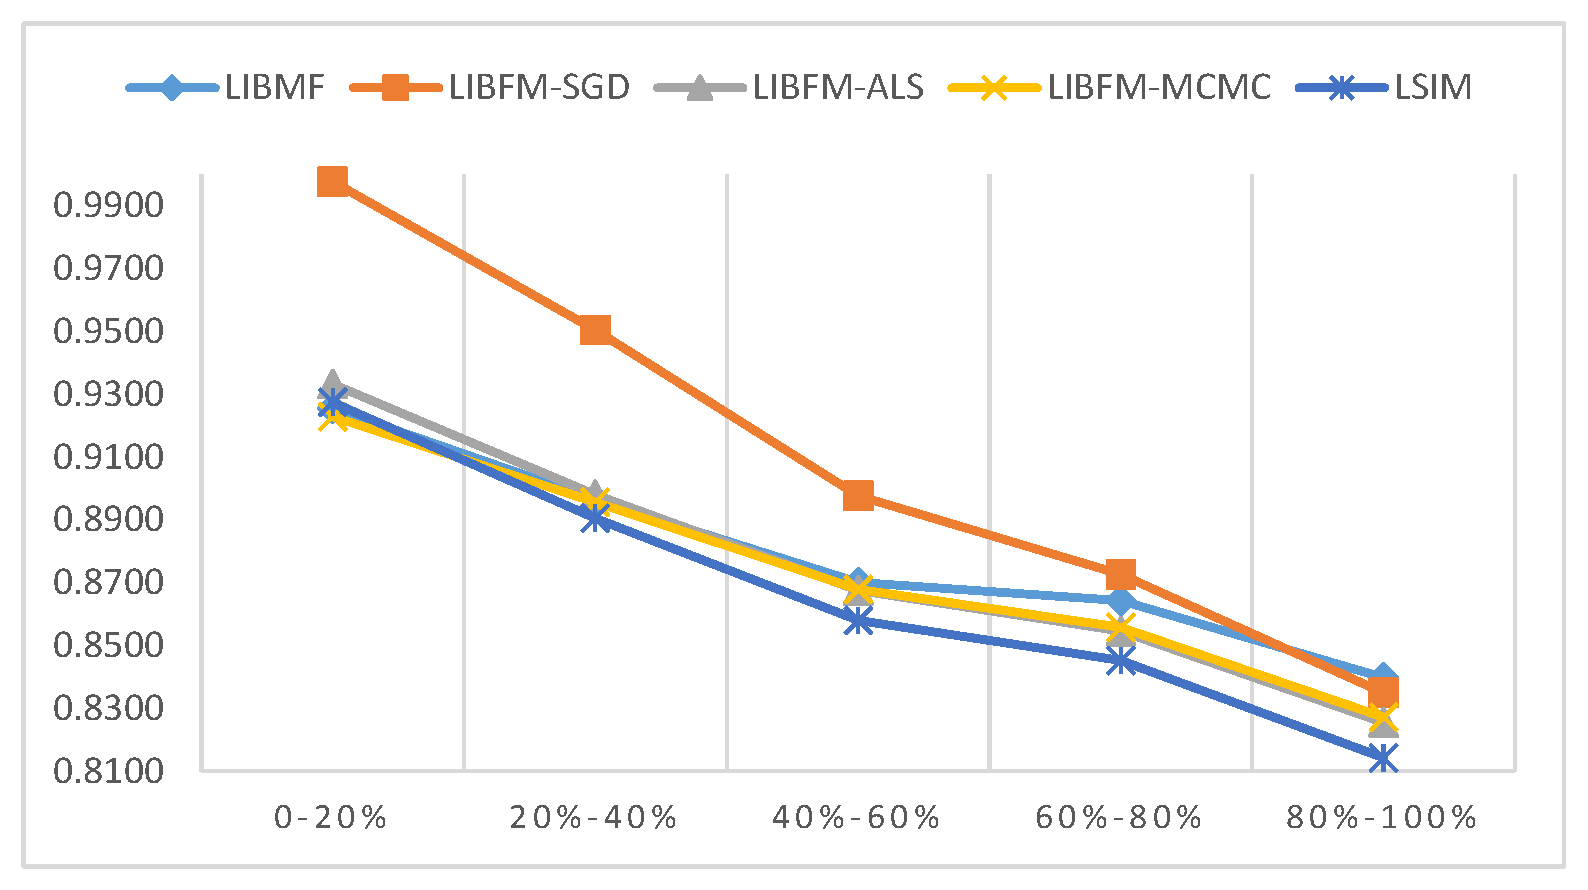
\includegraphics[scale=0.3]{images/rank_rmse.pdf}
    \caption{RMSE computed by cluster of users sorted by their respective number
    of ratings on MovieLens-10M with a training ratio of 90\%/10\%.}
    \label{fig:rank_rsme}
\end{figure}

\begin{figure}[htbp]
    \centering
    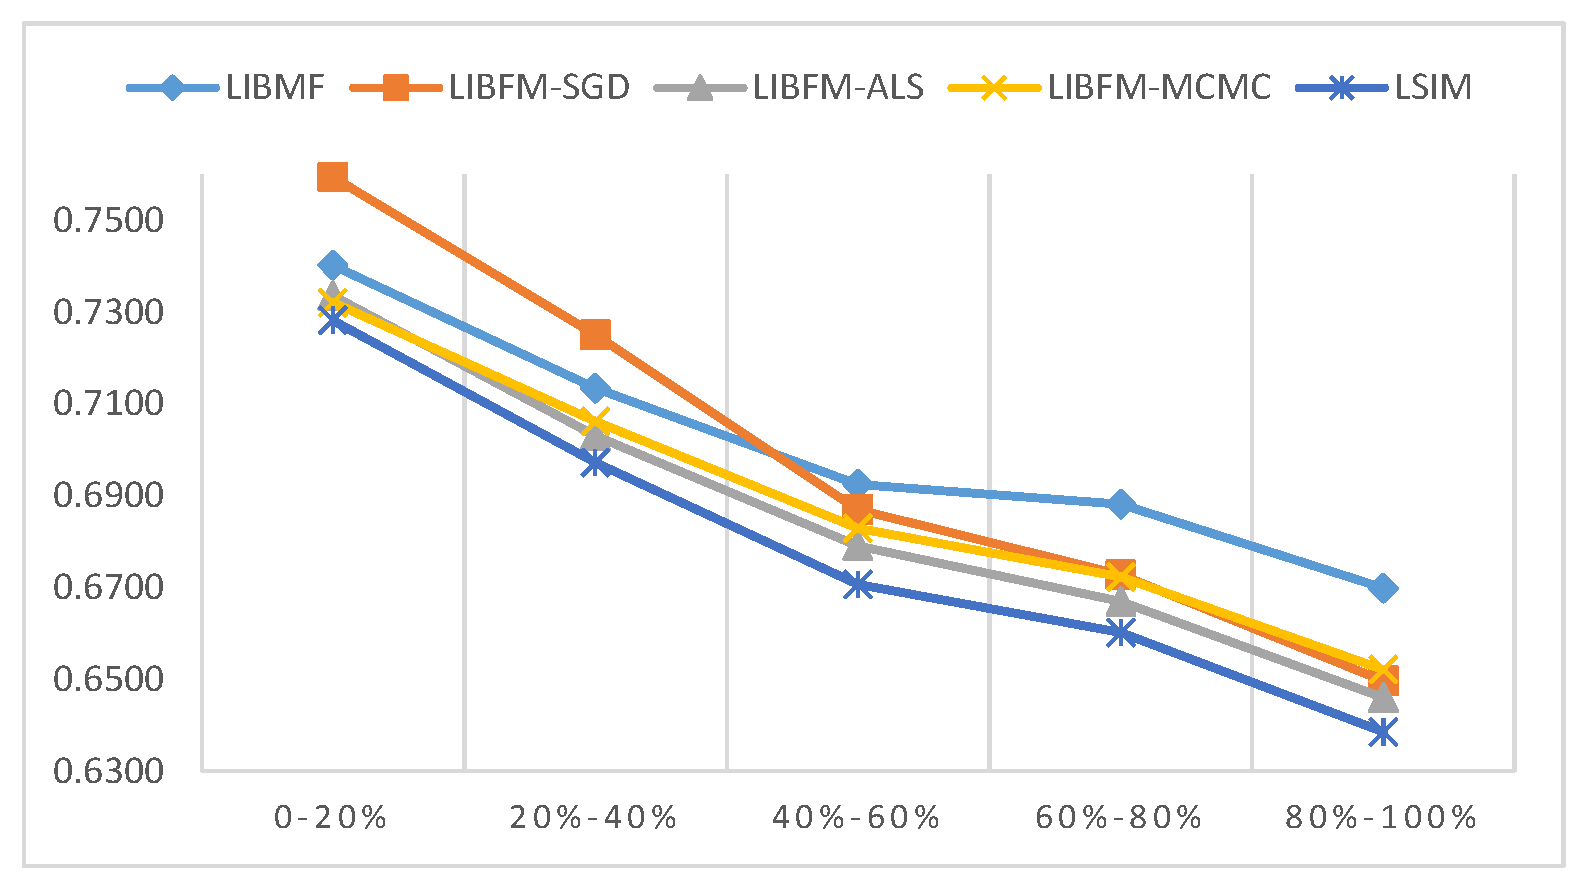
\includegraphics[scale=0.3]{images/rank_mae.pdf}
    \caption{MAE computed by cluster of users sorted by their respective number
    of ratings on MovieLens-10M with a training ratio of 90\%/10\%.}
    \label{fig:rank_mae}
\end{figure}

Figure \ref{fig:rank_rsme} shows the RMSE performance of all recommendation models
in different user clusters on MovieLens-1M dataset while Figure \ref{fig:rank_mae}
shows the MAE performance of all recommendation models in the same experimental
setting respectively.
It can be clearly observed from the two tables that all these recommendation models
benefit from the increase of the count of items the user interact with on both
RSME and MAE metrics.
Our proposed \textbf{LSIM} don't perform well at the first ``0\%-20\%'' user cluster,
its RMSE score is $0.9275$ which is less than \textbf{LibFM-MCMC}.
But when the interactions become more, its performance rapidly increases,
and beats the baseline methods obviously, which shows the effectiveness of our
long-short interest model.

\section{Conclusions and Future Works}
In this study, we propose to use long-short interest model to utilize the rich
sequential information on users interaction history to solve the rating
prediction task in recommender system.
By incorporating the sequential features into feature based collaborative
filtering framework, better prediction performance can be obtained.
Our thorough evaluation, using three standard MovieLens datasets, demonstrates
the effectiveness of the proposed method.

Many studies remain for the future work.
(1) When we carry out the long-short interest model, items given different ratings
are treated equally, and ratings information is ignored. Hence, how to take advantage
of the ratings information is one of our future works. 
(2) Side information plays an important role in recommender system, especially
for solving the cold start problem. In our long-short interest model, we don't use
any side information, but it is certain that with the help of side information,
users' long-short interest can be learned more effectively. Therefore, we will focus
on making use of side information in the future.

%\section{Acknowledgments}
%The work reported in this paper is supported by the National Natural
%Science Foundation of China Grant 61370116. We thank anonymous reviewers for
%their beneficial comments. We also thank Feifan Fan for valuable suggestions
%related to this paper.

\bibliographystyle{abbrv}
\bibliography{sigproc}

\end{document}
